\chapter{Selección y evaluación de núcleos TRNGs}		
	
	\section{Variación del reloj (Clock jitter)}
	
	Se supone que una señal de reloj ideal en los dispositivos lógicos digitales es una señal rectangular con un ciclo de trabajo del 50\% y un periodo estable. Pero debido a los diversos ruidos que afectan a los dispositivos electrónicos, la señal de reloj nunca es absolutamente estable y sus flancos se mueven de su posición estable. En otras palabras, la fase de la señal de reloj fluctúa. Esta fluctuación puede verse como una variación del reloj en el dominio del tiempo y como un ruido de fase en el dominio de la frecuencia. En los dispositivos lógicos, una variación del reloj suele ser indeseado, pero inevitable. Dado que estas variaciones afectan negativamente a las comunicaciones de alta frecuencia y a los sistemas de alta velocidad, ha sido bien estudiado y caracterizado.
	
	En los sistemas analógicos, el jitter se caracteriza mejor en el dominio de la frecuencia. De este modo, los componentes de fase y amplitud pueden estudiarse y caracterizarse por separado. En cambio, en los sistemas digitales, las propiedades temporales del jitter son más importantes y, por tanto, el jitter se caracteriza en el dominio del tiempo.
	
	Las variaciones del reloj en un sistema digital es una desviación del flanco de reloj real con respecto a un flanco de reloj ideal. Una señal de reloj ideal se define mediante la ecuación (\ref{eq:periodic}), donde $t(n)$ representa el tiempo del $n$-ésimo periodo de una señal de reloj y $T$ es el periodo de una señal de reloj.
	
	\begin{equation}
		t(n) =  n T
	\label{eq:periodic}
	\end{equation}
	
	Una señal de reloj real no llega siempre a múltiplos enteros de su periodo, como lo hace la ideal, sino que sus flancos fluctúan en torno a este valor a causa del jitter. El jitter está causado por diversos fenómenos físicos, como el ruido térmico, el ruido de la fuente de alimentación, el ruido electromagnético ambiental, etc.	
	
	
	
	\section{Arquitectura de núcleos TRNG seleccionados}

	Con base en los criterios del AIS-20/31, y los núcleos \gls{TRNG} que usan estructuras oscilantes como se clasifican en \cite{Petura2016}:
	
	\begin{itemize}
		\item Single-event ring oscillators
			\begin{itemize}
				\item Elementary ring oscillator based TRNG (\gls{ERO-TRNG})
				\item Coherent sampling ring oscillator based TRNG (\gls{COSO-TRNG})
				\item Multi-ring oscillator based TRNG (\gls{MURO-TRNG})
			\end{itemize}
		\item Multi-event ring oscillators with signal collisions
			\begin{itemize}
				\item Transient effect ring oscillator based TRNG (\gls{TERO-TRNG})
			\end{itemize}
		\item Multi-event ring oscillators without signal collisions
			\begin{itemize}
				\item Self-timed ring based TRNG (\gls{STR-TRNG})
			\end{itemize}
		\item Phase-locked loops
			\begin{itemize}
				\item PLL based TRNG (\gls{PLL-TRNG})
			\end{itemize}
	\end{itemize}
	
		\subsection{Elementary ring oscillator based TRNG (ERO-TRNG)}
		
					
				\begin{figure}[hbtp]
					\caption{Arquitectura del núcleo ERO-TRNG.}
					\centering
					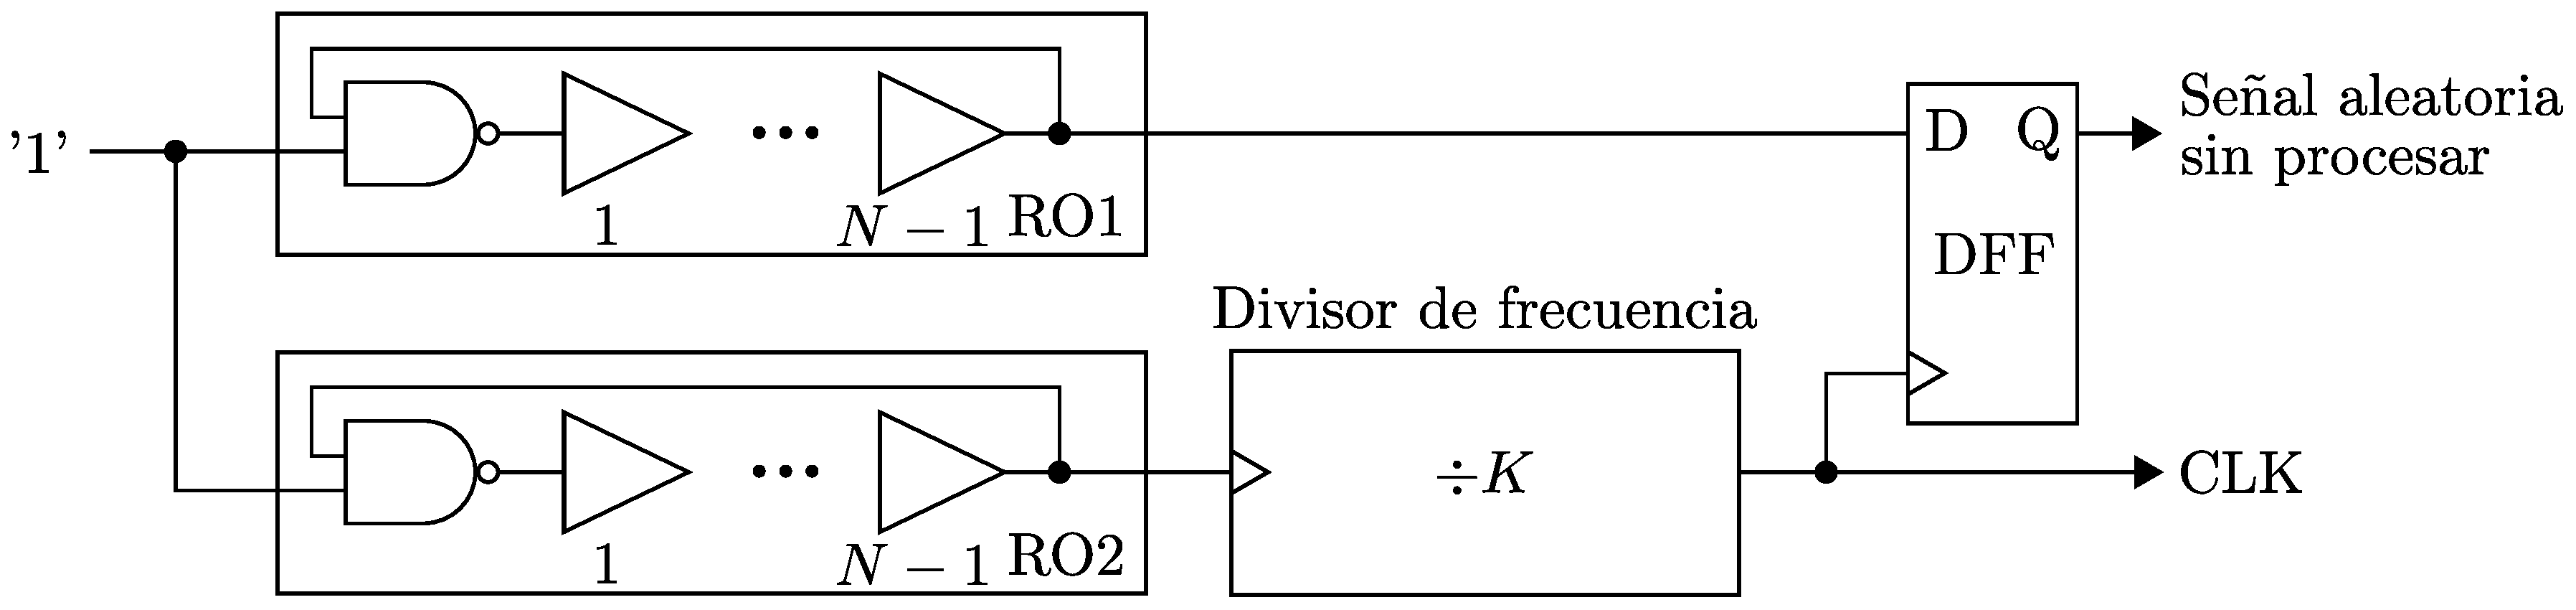
\includegraphics[width=0.8\linewidth]{A1_ERO_TRNG}
					\label{fig:A1_ERO_TRNG}
				\end{figure}
			
			
			
		\subsection{Coherent sampling ring oscillator based TRNG (COSO-TRNG)}
	
				
				\begin{figure}[hbtp]
					\caption{Arquitectura del núcleo COSO-TRNG.}
					\centering
					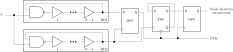
\includegraphics[width=0.8\linewidth]{A2_COSO_TRNG}
					\label{fig:A2_COSO_TRNG}
				\end{figure}
				
				
				
		\subsection{Multi-ring oscillator based TRNG (MURO-TRNG)}
	
				
				\begin{figure}[hbtp]
					\caption{Arquitectura del núcleo MURO-TRNG.}
					\centering
					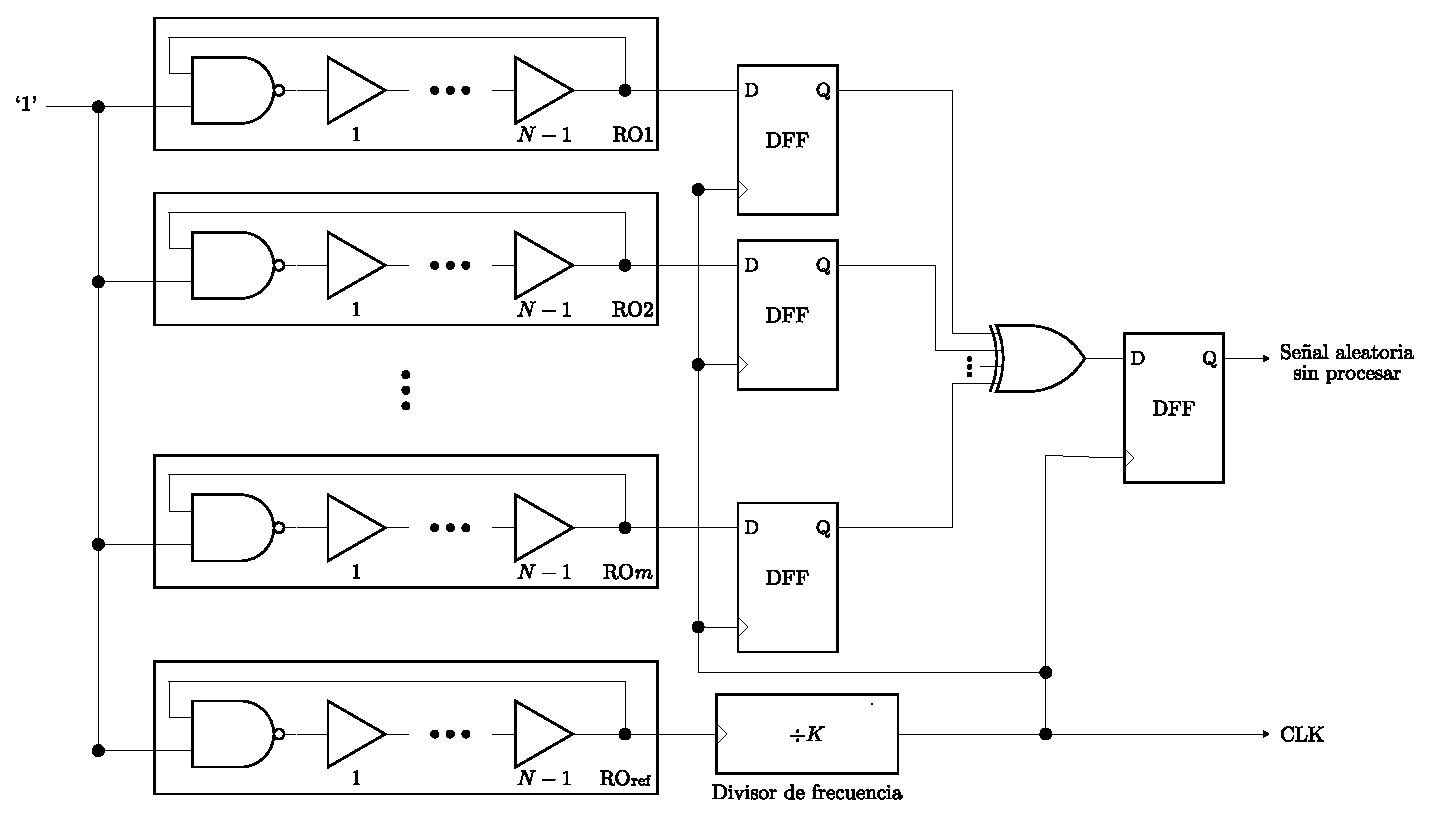
\includegraphics[width=0.8\linewidth]{A3_MURO_TRNG}
					\label{fig:A3_MURO_TRNG}
				\end{figure}
				
				
				
		\subsection{Transient effect ring oscillator based TRNG (TERO-TRNG)}
	
				
				\begin{figure}[hbtp]
					\caption{Arquitectura del núcleo TERO-TRNG.}
					\centering
					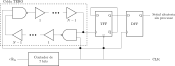
\includegraphics[width=0.8\linewidth]{A4_TERO_TRNG}
					\label{fig:A4_TERO_TRNG}
				\end{figure}
				
				
				
		\subsection{Self-timed ring based TRNG (STR-TRNG)}
	
				
				\begin{figure}[hbtp]
					\caption{Arquitectura del núcleo STR-TRNG.}
					\centering
					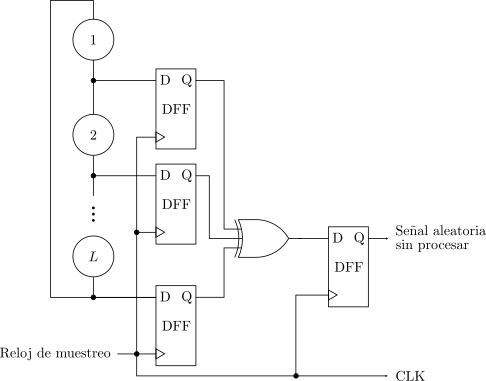
\includegraphics[width=0.8\linewidth]{A5_STR_TRNG}
					\label{fig:A5_STR_TRNG}
				\end{figure}
				
				
				
		\subsection{PLL based TRNG (PLL-TRNG)}
	
				
				\begin{figure}[hbtp]
					\caption{Arquitectura del núcleo PLL-TRNG.}
					\centering
					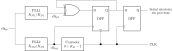
\includegraphics[width=0.8\linewidth]{A6_PLL_TRNG}
					\label{fig:A6_PLL_TRNG}
				\end{figure}
				
				
			
		   



% Table generated by Excel2LaTeX from sheet 'Sheet1'
\begin{table}[htbp]
  \centering
  \caption{Resumen de los resultados de implementación de las TRNGs}
\resizebox{0.8\linewidth}{!}{ 
    \begin{tabular}{|c|c|c|c|c|c|c|c|c|}
    \hline
    \rowcolor[rgb]{ .682,  .667,  .667} TRNG Type & FPGA  & Area  & Power cons. & Bit Rate & Efficiency & Entropy & Entropy * Bit rate & Feasib. \\
    \rowcolor[rgb]{ .682,  .667,  .667}       & device & (LUT/Reg) & [mW]  & [Mbits/s] & [bits/$\mu$Ws] & per bit &       & \& Repeat. \\
    \hline
    \multirow{3}[2]{*}{ERO} & Spartan 6 & 46/19 & 2.16  & 0.0042 & 1.94  & 0.999 & 0.004 & \multirow{3}[2]{*}{5} \\
          & Cyclone V & 34/20 & 3.24  & 0.0027 & 0.83  & 0.990 & 0.003 &  \\
          & SmartFusion 2 & 45/19 & 4     & 0.014 & 3.5   & 0.980 & 0.013 &  \\
    \hline
    \multirow{3}[2]{*}{COSO} & Spartan 6 & 18/3  & 1.22  & 0.54  & 442.6 & 0.999 & 0.539 & \multirow{3}[2]{*}{1} \\
          & Cyclone V & 13/3  & 0.9   & 1.44  & 1600  & 0.999 & 1.438 &  \\
          & SmartFusion 2 & 23/3  & 1.94  & 0.328 & 169   & 0.999 & 0.327 &  \\
    \hline
    \multirow{3}[2]{*}{MURO} & Spartan 6 & 521/131 & 54.72 & 2.57  & 46.9  & 0.999 & 2.567 & \multirow{3}[2]{*}{4} \\
          & Cyclone V & 525/130 & 34.93 & 2.2   & 62.9  & 0.999 & 2.197 &  \\
          & SmartFusion 2 & 545/130 & 66.41 & 3.62  & 54.5  & 0.999 & 3.616 &  \\
    \hline
    \multirow{3}[2]{*}{PLL} & Spartan 6 & 34/14 & 10.6  & 0.44  & 41.5  & 0.981 & 0.431 & \multirow{3}[2]{*}{3} \\
          & Cyclone V & 24/14 & 23    & 0.6   & 43.4  & 0.986 & 0.592 &  \\
          & SmartFusion 2 & 30/15 & 19.7  & 0.37  & 18.7  & 0.921 & 0.340 &  \\
    \hline
    \multirow{3}[2]{*}{TERO} & Spartan 6 & 39/12 & 3.312 & 0.625 & 188.7 & 0.999 & 0.624 & \multirow{3}[2]{*}{1} \\
          & Cyclone V & 46/12 & 9.36  & 1     & 106.8 & 0.987 & 0.985 &  \\
          & SmartFusion 2 & 46/12 & 1.23  & 1     & 813   & 0.999 & 0.999 &  \\
    \hline
    \multirow{3}[2]{*}{STR} & Spartan 6 & 346/256 & 65.9  & 154   & 2343.2 & 0.998 & 154.121 & \multirow{3}[2]{*}{2} \\
          & Cyclone V & 352/256 & 49.4  & 245   & 4959.1 & 0.999 & 244.755 &  \\
          & SmartFusion 2 & 350/256 & 82.52 & 188   & 2286.7 & 0.999 & 188.522 &  \\
    \hline
    \end{tabular}%
}
  \label{tab:addlabel}%

\end{table}%


\gls{FPGA}.

\gls{RNG}.


\gls{TERO}.


	 
	
	
	
